\begin{figure}[htbp]
\centering
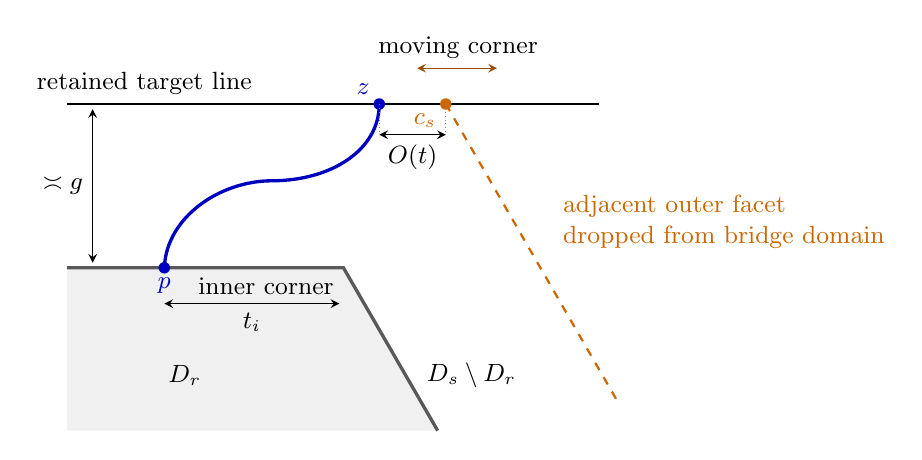
\begin{tikzpicture}[scale=1.3,>=stealth,font=\small]
 \fill[gray!12] (-2.7,0)--(0,0)--(.92,-1.59)--(-2.7,-1.59)--cycle;
 \draw[gray!70!black,very thick] (-2.7,0)--(0,0)--(.92,-1.59);
 \node at (-1.55,-1.05) {$D_r$};
 \node at (1.25,-1.05) {$D_s\setminus D_r$};
 \node[below left] at (0,0) {inner corner};
 \draw[thick] (-2.7,1.6)--(2.5,1.6);
 \node[above left] at (-.8,1.6) {retained target line};
 \draw[orange!80!black,thick,dashed] (1,1.6)--(2.7,-1.344);
 \draw[orange!60!black,<->] (.72,1.95)--(1.5,1.95);
 \node[above] at (1.12,1.95) {moving corner};
 \node[orange!80!black,align=left,anchor=west] at (2.05,.45)
   {adjacent outer facet\\dropped from bridge domain};
 \fill[orange!80!black] (1,1.6) circle(1.6pt) node[below left] {$c_s$};
 \draw[blue!75!black,very thick] (-1.75,0)
   .. controls (-1.73,.5) and (-1.2,.85) .. (-.7,.85)
   .. controls (-.12,.85) and (.35,1.15) .. (.35,1.6);
 \fill[blue!75!black] (-1.75,0) circle(1.6pt) node[below] {$p$};
 \fill[blue!75!black] (.35,1.6) circle(1.6pt) node[above left] {$z$};
 \draw[<->] (.35,1.3)--(1,1.3) node[midway,below] {$O(t)$};
 \draw[gray,densely dotted] (.35,1.6)--(.35,1.3);
 \draw[gray,densely dotted] (1,1.6)--(1,1.3);
 \draw[<->] (-1.75,-.35)--(-.04,-.35) node[midway,below] {$t_i$};
 \draw[<->] (-2.45,.05)--(-2.45,1.55) node[midway,left] {$\asymp g$};
\end{tikzpicture}
\caption{The selected band bridge from an inner port $p$ to an outer port $z$, with $g=s-r$. The inner elbow is retained when bounding the bridge, while the dashed adjacent outer facet is dropped. After fixing the target support, the adjacent support is still independent and has conditional density, or row-atom bound, $O(1/g)$. Its intersection $c_s$ with the target therefore falls within $O(t)$ of a fixed $z$ with probability at most $C\min(1,t/(1+g))$, including row rounding. The diagram is schematic; the second band bridge is bounded uniformly without revealing this support.}
\label{fig:sewing-band}
\end{figure}
